\begin{figure}[h!]
\centering
\caption{Pago de intereses del GNC}
\label{fig:Intereses}
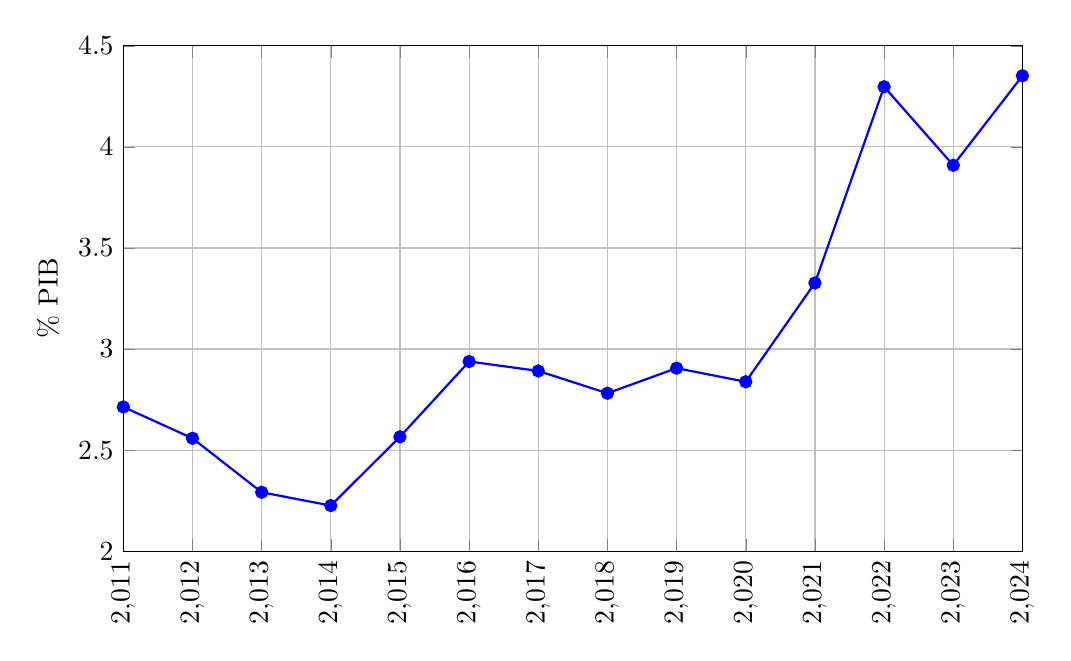
\begin{tikzpicture}
\begin{axis}[
    width=13cm, height=8cm,
    %title={Intereses (\% PIB)},
    %xlabel={A\~nos},
    ylabel={\% PIB},
    ymin=2, ymax=4.5,
%    xmin=2004, xmax=2024,
    xmin=2011, xmax=2024,
    x tick label style={rotate=90, anchor=east},
    grid=major,
    legend style={at={(0.5,-0.14)}, anchor=north, legend columns=-1},
    legend cell align={left}
    every tick label/.append style={
    /pgf/number format/.cd,
    use period, % Forces the use of a period as decimal separator
    1000 sep={}, % Removes thousands separator
    fixed}
]
% Intereses
\addplot[solid, thick, blue, mark=*] table {
%2004	3.59624495
%2005	3.11178406
%2006	3.659407384
%2007	3.712500323
%2008	3.224309743
%2009	3.020318995
%2010	2.728931009
2011	2.713678894
2012	2.558460496
2013	2.291506951
2014	2.225634705
2015	2.565679095
2016	2.938439479
2017	2.891665921
2018	2.781357961
2019	2.905510743
2020	2.837994172
2021	3.326883193
2022	4.29753116
2023	3.909045017
2024	4.351706393
};
\end{axis}
\end{tikzpicture}
\par \footnotesize{\textit{Fuente: \textcite{minhacienda_balance_2025}}}
\end{figure}

